% --- chapter
\newcommand{\chapter}[2][]{
	\newcommand{\chapname}{#2}
	\begin{flushleft}
		\begin{minipage}[t]{\linewidth}
			
\includegraphics[height=1cm]{hdht-logo.png}
			\hspace{0pt}	
			\sffamily\bfseries\large Bài  25. Giao thoa ánh sáng
			\begin{flushleft}
				\huge\bfseries #1
			\end{flushleft}
		\end{minipage}
	\end{flushleft}
	\vspace{1cm}
	\normalfont\normalsize
}
%-----------------------------------------------------
\chapter[Giao thoa ánh sáng và điều kiện xảy ra giao thoa ánh sáng]{Giao thoa ánh sáng \\và điều kiện xảy ra giao thoa ánh sáng}

\subsection{Hiện tượng nhiễu xạ ánh sáng}
Hiện tượng truyền sai lệch so với sự truyền thẳng khi ánh sáng gặp vật cản gọi là hiện tượng nhiễu xạ ánh sáng.

Hiện tượng nhiễu xạ chỉ có thể giải thích được nếu thừa nhận ánh sáng có tính chất sóng. Mỗi ánh sáng đơn sắc coi như một sóng có bước sóng xác định.
\begin{center}
	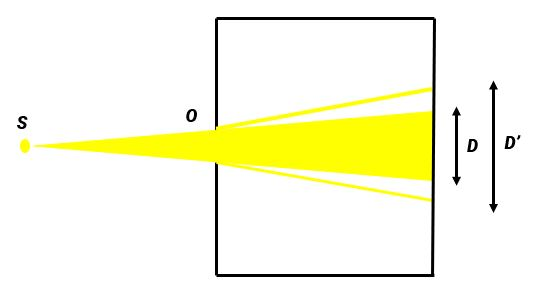
\includegraphics[scale=0.7]{../figs/VN12-PH-33-L-020-1-2.JPG}
\end{center}

\subsection{Hiện tượng giao thoa ánh sáng}
\begin{description}
	\item[Hiện tượng giao thoa ánh sáng] là hiện tượng hai chùm ánh sáng kết hợp khi chồng lên nhau sẽ tạo ra những chỗ chúng tăng cường lẫn nhau, và những chỗ chúng triệt tiêu lẫn nhau tạo ra những vân sáng, vân tối xen kẽ nhau. 
	
	Hiện tượng giao thoa ánh sáng là một bằng chứng thực nghiệm quan trọng khẳng định ánh sáng có tính chất sóng.
	\item[Hai nguồn sáng kết hợp] là hai nguồn sáng  phát ra hai sóng ánh sáng có cùng bước sóng và hiệu số pha dao động giữa hai nguồn không thay đổi theo thời gian.
	\item[Điều kiện xảy ra giao thoa ánh sáng] là hai chùm sáng giao nhau phải là hai chùm sáng kết hợp.
\end{description}



\subsection{Vị trí các vân}
Ta ký hiệu: 
\begin{itemize}
	\item $a$ là khoảng cách giữa hai nguồn kết hợp,
	\item $D$ là khoảng cách từ hai nguồn đến màn,
	\item $\lambda$ là bước sóng ánh sáng,
	\item $x$ là tọa độ của điểm đang xét trên màn.
\end{itemize}
\begin{center}
	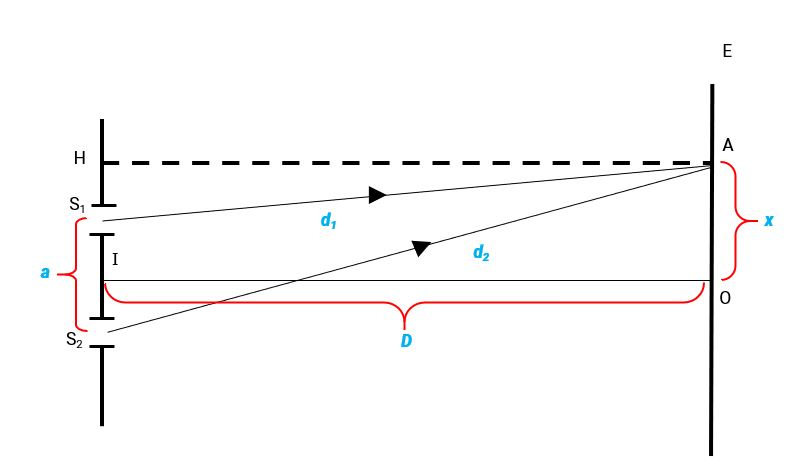
\includegraphics[scale=0.7]{../figs/VN12-PH-33-L-020-1-1.JPG}
\end{center}

\subsubsection{Hiệu quang lộ và vân giao thoa}
	 Hiệu đường đi $\delta$ trong trường hợp $a\ll D$:
		\begin{equation}
			\delta = d_2-d_1=\dfrac{ax}{D}.  
		\end{equation}
	Tính chất vân tại A phụ thuộc hiệu quang lộ:
	\begin{itemize}
		\item Để tại A là vân sáng thì: $$d_2-d_1=k\lambda$$ với $k=0; \pm 1; \pm 2,...$
	 	\item Để tại A là vân tối: $$d_2-d_1=\left(k+\dfrac{1}{2}\right) \lambda$$ với $k= \pm 1; \pm 2,...$
	\end{itemize}
\subsubsection{Vị trí vân sáng và vân tối}
	Vị trí vân sáng:
	\begin{equation}
		 x=k\dfrac{\lambda D}{a},\ k=\pm 1; \pm 2,...
	 \end{equation}
	 
	Vị trí vân tối: 
	\begin{equation}
		x=\left(k'+\dfrac{1}{2}\right) \dfrac{\lambda D}{a},\ k'=0; \pm 1; \pm 2,... 
	\end{equation}


\subsubsection{Khoảng vân}
Khoảng vân $i$ là khoảng cách giữa hai vân sáng, hoặc hai vân tối liên tiếp.

Công thức tính khoảng vân: 
\begin{equation}\label{eq:khoangvan}	
	i=\dfrac{\lambda D}{a}.	
\end{equation}
	
Tại O là vân sáng bậc 0 của mọi bức xạ chính là vân chính giữa hay vân trung tâm.

\subsubsection {Ứng dụng đo bước sóng ánh sáng}
Trong thí nghiệm giao thoa với khe Young, bằng cách đo $i$, $a$, $D$, bước sóng ánh sáng $\lambda$ được suy ra từ công thức \eqref{eq:khoangvan}.
